\section{Time complexities}
\label{sec:time_complexities}

\begin{frame}
	\frametitle{How long does this all take?}
	
	\begin{center}
		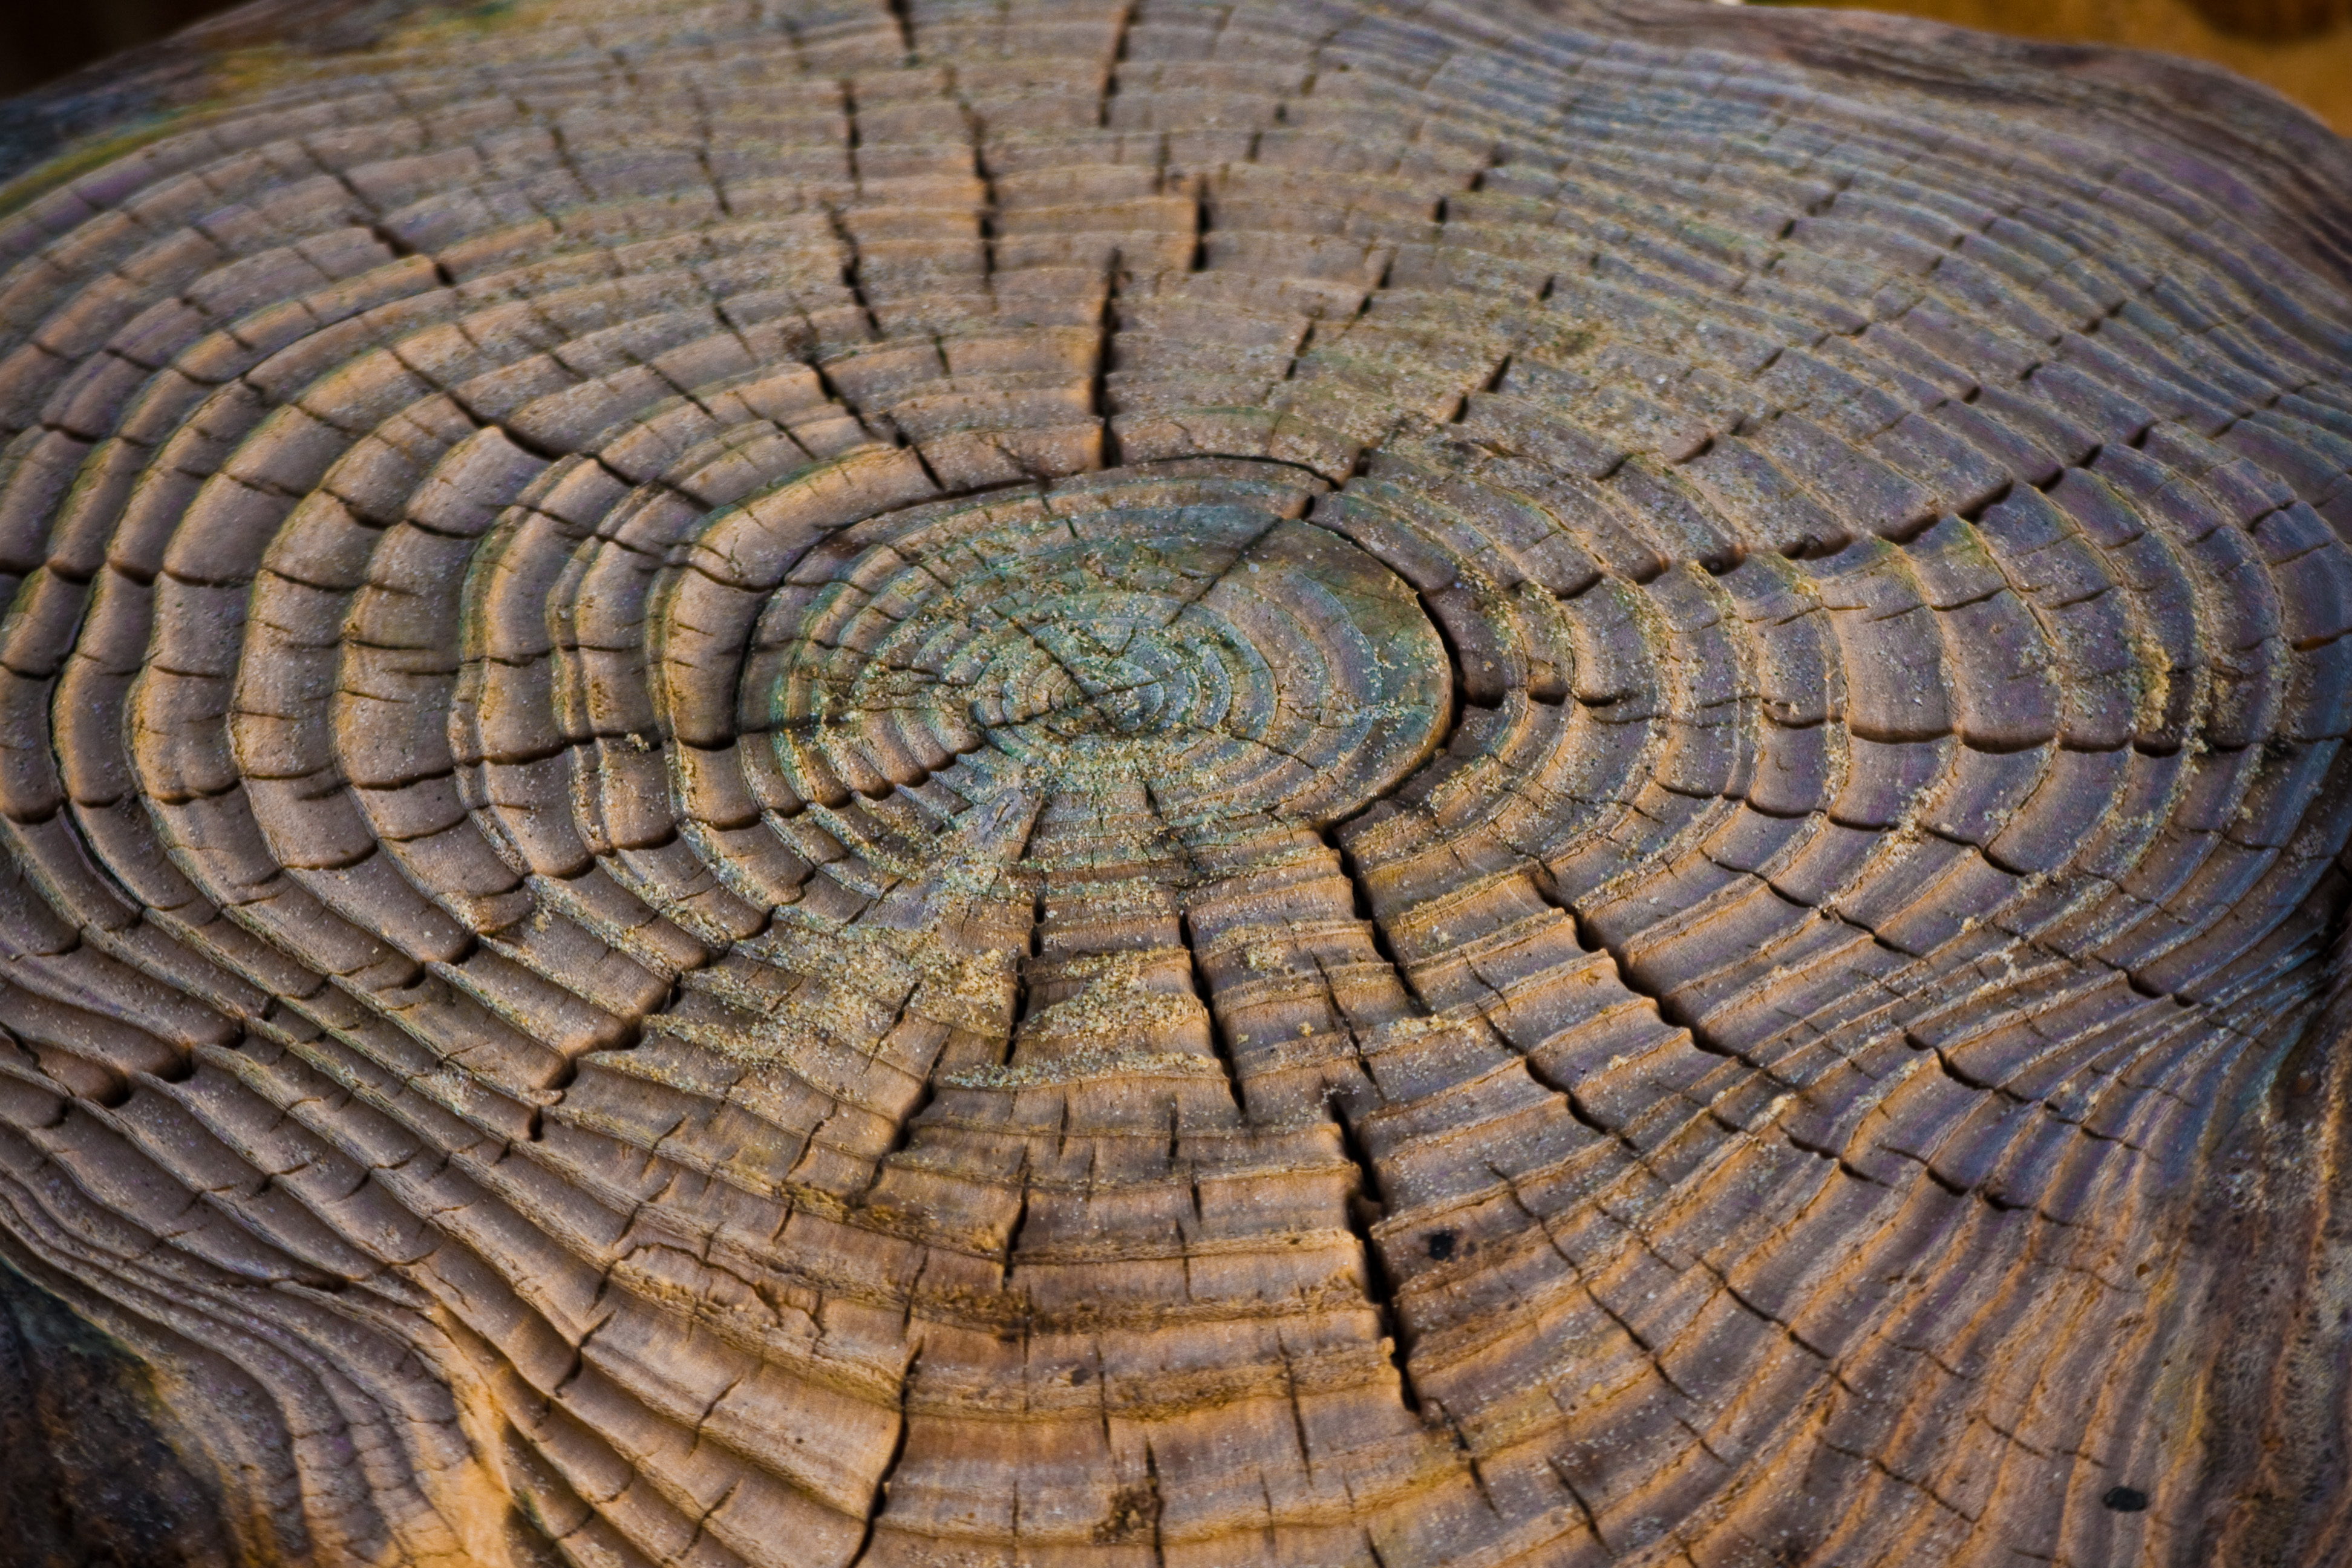
\includegraphics[width=0.6\textwidth]{figures/tree_age.jpg}\\
		\hspace*{15pt}\hbox{\scriptsize Image By:\thinspace{\itshape Garry Knight}}
		% https://www.flickr.com/photos/garryknight/3829280573
	\end{center}
\end{frame}

\begin{frame}
	\frametitle{Expressing time complexity}
	\begin{questionblock}{How can we express the time of Tree operations?}
		For operations like \texttt{height} and \texttt{depth} what is the time complexity?
	\end{questionblock}
	\pause
		\begin{block}{Two parameters}
			For functions on trees, we consider two parameters:
			\begin{itemize}
				\item $n$ the number of nodes in the tree.
				\item $h$ the height of the tree.
			\end{itemize}
		\end{block}	
\end{frame}

\begin{frame}
	\frametitle{Alternative implementation: Node Depth}
	
	\lstinputlisting{code/tree_alt_depth.py}
	\begin{questionblock}{What do we do?}
		What is the time complexity of this function?\\
		Note: this uses the implementation wher every node is a subtree itself.
		\only<2>{
		\begin{multicols}{2}
			\begin{enumerate}[A.]
				\item $\Theta(h)$
				\item $\Theta(h^2)$
				\item $\Theta(n)$
				\item $\Theta(n^2)$
			\end{enumerate}
		\end{multicols}
	}
	\end{questionblock}
	\only<3>{
	\begin{answerblock}{Like sending a hobbit up a tree}
		We only consider one path straight to the top, so this is $O(h)$.
	\end{answerblock}
}
\end{frame}

\begin{frame}
	\frametitle{Alternative implementation: Tree Height}
	\lstinputlisting{code/tree_alt_height.py}
	\begin{questionblock}{What do we do?}
		What is the time complexity of this function?\\
		Note: this uses the implementation wher every node is a subtree itself.
		\only<2>{
		\begin{multicols}{2}
			\begin{enumerate}[A.]
				\item $\Theta(h)$
				\item $\Theta(h^2)$
				\item $\Theta(n)$
				\item $\Theta(n^2)$
			\end{enumerate}
		\end{multicols}
	}
	\end{questionblock}
	\only<3>{
	\begin{answerblock}{Some kind of irony}
		Worst case we need to check all nodes, so $O(n)$ to determine $h$.
	\end{answerblock}
}
\end{frame}


